\scanpage{63}\mspage{62}
En effet, $G=G'\amalg G''$ ou $G'\subset F',G''\subset F''$, \deleted{$G'$ et $G''$ disjoints,} \inserted{(cf p. 57)} donc on a $G'=\unsure{G|e|\phi|0}$ ou $G''=G$. donc $G\subset F'$ ou $G\subset F''$ qed.

\uline{Corollaire} 1 \deleted{Deux} Soient $F_0,F_1$ deux comp. connexes de $F$. Alors \unsure{on a|ou} $F_0=F_1$ ou $F_0$ et $F_1$ sont disjoints, et \deleted{\unsure{alors}} \inserted{dans ce cas} $F=F_0\amalg F_1\amalg \deleted{\unsure{G|F}}H$

\margin{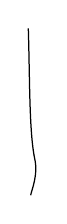
\begin{tikzpicture}[x=1cm,y=1cm]\draw[line width=.45pt] (0,0) .. controls (.02,-.65) and (.01,-1.3) .. (.08,-1.65) .. controls (.13,-1.86) and (.04,-2.06) .. (.03,-2.12);\end{tikzpicture}}

On écrit $F=F_0\amalg G$, et on applique \unsure{lemme|Lemme}

\deleted{\uline{Corollaire 2} Soit $(F_i)_{\unsure{\nu|j|i}\in I}$ une famille de composantes connexes deux \unsure{;|à} deux disjointes. Alors \deleted{$F\unsure{=}\coprod F_{\unsure{i}}$} la figure \unsure{engendrée|engendree} par les $F_i$ est leur somme disjointe $\coprod F_i$ \deleted{\unsure{et}} $\subset F$, et si \unsure{la|le} famille est finie (p. ex. $F$ \deleted{fini} figure finie) alors $F=(\coprod F_i)\amalg H$\unsure{.|,}

\unsure{Il|Je} n'est pas \unsure{évident|evident} que tte figure non vide ait une composante connexe, \deleted{\unsure{la|le} \unsure{difficulté|fait} \unsure{étant} dans \unsure{l'existence|les fig.} \unsure{ou}} \deleted{\unsure{à|a} des sous-figures \unsure{``compl. dis''|``complém.res''|``comprises''|``complètes''}} \inserted{Mais c'est \unsure{vrai} pour les figures de \unsure{t.f.|s.fg.|S.fg.}, et a fortiori pour les figures finies. Les}}

\uline{Proposition} Soit $F$ une figure, $A=\overline F\inserted{\subset M}$ l'ens de ses \unsure{strates.|str. loc.|str. lin.} \deleted{Alors l'application\unsure{,}} Pour qu'une sous-figure \deleted{$F$} $F_0$ de $F$ soit une comp. conn. de $F$, il f et s que $\overline{F_0}$ soit une composante connexe de l'ens. ordonné $A$ (pour l'ordre induit par $\leq$). On trouve ainsi une corr. biunivoque entre l'ens. \unsure{de|des} comp. conn.
